\section[گام ششم: انتخاب رویکرد و مدل]{\faProjectDiagram\ \ گام ششم: انتخاب رویکرد و مدل}
\begin{stepbox}

\field{انتخاب نوع مدل}{
    رویکرد مناسب برای این مسئله، یادگیری عمیق (\lr{Deep Learning}) است. روش‌های کلاسیک پردازش تصویر، مانند آستانه‌گذاری (\lr{Thresholding})، و نیز الگوریتم‌های سنتی یادگیری ماشین، توانایی کافی برای مدل‌سازی الگوهای پیچیده، سه‌بعدی و غیرخطی موجود در بافت‌های نرم و مرزهای مبهم تومورها در تصاویر \lr{CT} را ندارند. در مقابل، شبکه‌های عمیق می‌توانند ویژگی‌های سطح پایین و سطح بالا را به‌صورت خودکار استخراج کرده و برای مسئله بخش‌بندی پزشکی عملکرد به‌مراتب دقیق‌تری ارائه دهند.
}

\field{انتخاب الگوریتم یا معماری مناسب}{
    برای وظایف بخش‌بندی تصاویر پزشکی، معماری‌های مبتنی بر \lr{U-Net} به‌عنوان یک استاندارد شناخته می‌شوند. در این پروژه، با توجه به شواهد پژوهشی و نتایج گزارش‌شده در مقالات جدید، استفاده از معماری \lr{UNet++} پیشنهاد می‌شود. این معماری با بهره‌گیری از مسیرهای پرش متراکم (\lr{Dense Skip Connections})، شکاف معنایی میان ویژگی‌های لایه‌های رمزگذار و رمزگشا را کاهش می‌دهد و امکان ترکیب بهتر اطلاعات مکانی و معنایی را در سطوح مختلف فراهم می‌کند.
}
\newpage
\begin{center}
    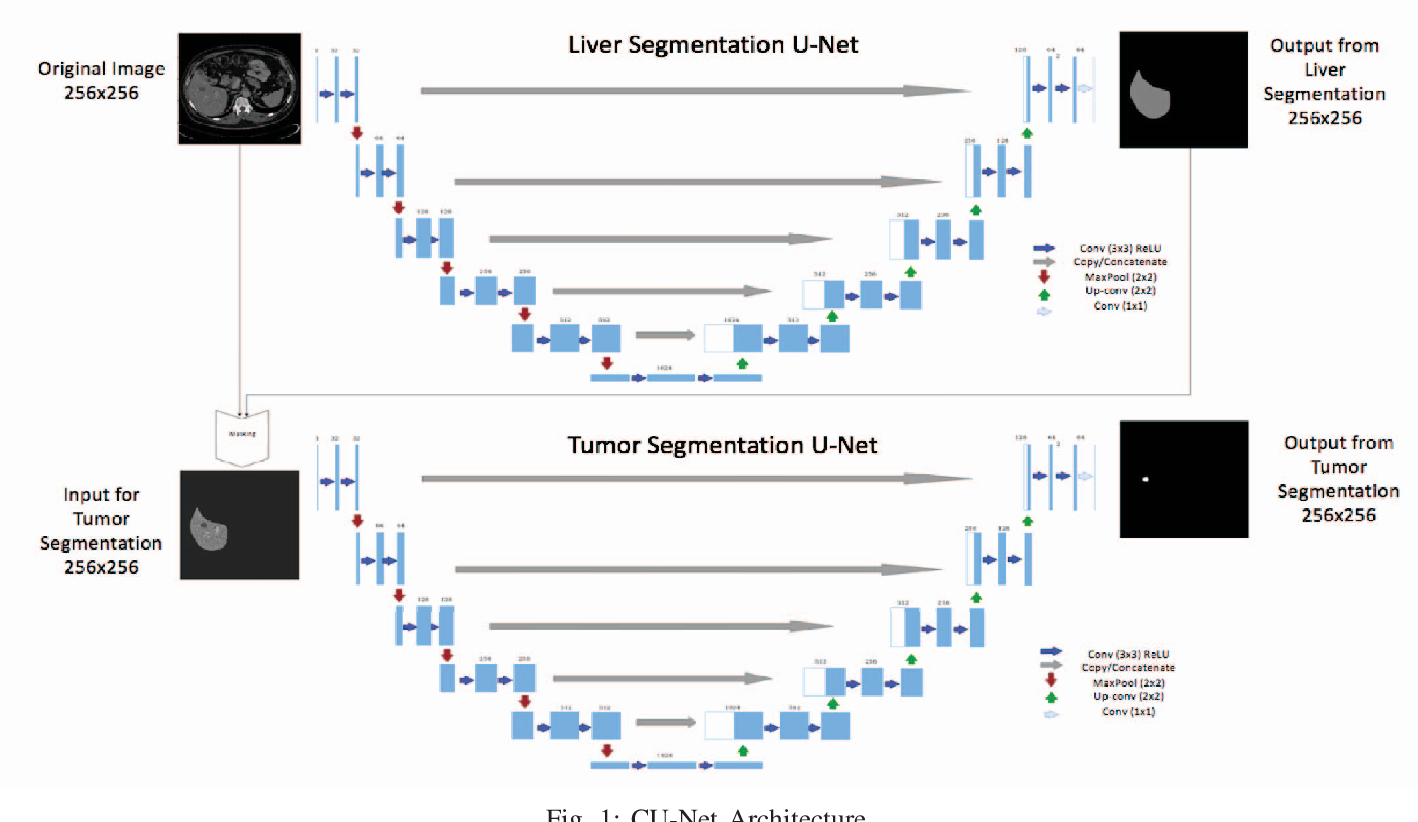
\includegraphics[width=0.85\textwidth]{images/liver-and-tumor-unet-segmentation.png}
    \vspace{0.2cm} \\
    \footnotesize{شکل ۶ - شماتیک معماری \lr{Cascaded U-Net} (شبکه‌های آبشاری) برای بخش‌بندی مرحله‌به‌مرحله کبد و تومور.}
\end{center}



\field{استفاده از مدل‌های از پیش آموزش‌دیده یا مدل سفارشی}{
    آموزش کامل مدل از صفر (\lr{From Scratch}) در حوزه پزشکی، به دلیل محدودیت حجم داده‌های برچسب‌خورده، معمولاً انتخاب بهینه‌ای نیست. رویکرد مناسب‌تر، استفاده از یادگیری انتقالی (\lr{Transfer Learning}) است. در این روش، یک شبکه از پیش آموزش‌دیده مانند \lr{ResNet} یا \lr{EfficientNet} به‌عنوان بخش استخراج‌کننده ویژگی (\lr{Encoder Backbone}) در ساختار \lr{UNet++} به کار گرفته می‌شود و سپس وزن‌های آن متناسب با داده‌های تخصصی پروژه، مانند دیتاست \lr{LiTS}، به‌صورت تنظیم ظریف (\lr{Fine-tuning}) بهینه می‌گردد.
}

\end{stepbox}
